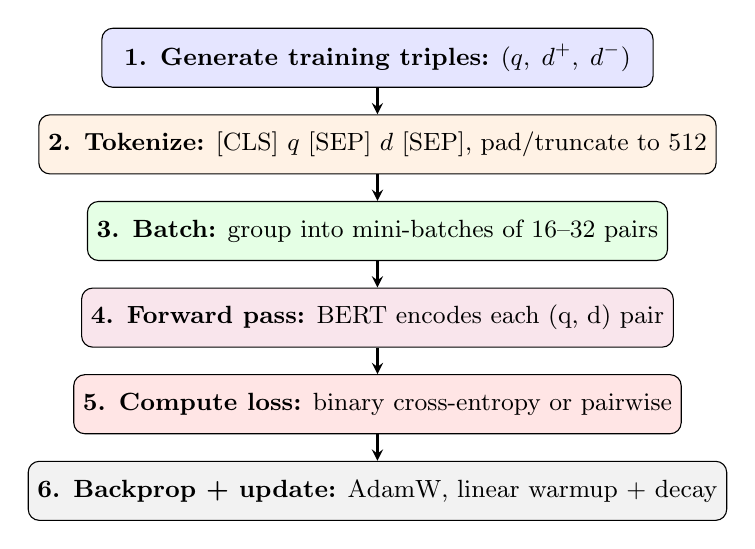
\begin{tikzpicture}[
    node distance=1.1cm,
    box/.style={rectangle, draw, rounded corners, minimum width=7cm, minimum height=0.75cm, align=center, font=\small},
    arrow/.style={->, thick, >=stealth}
]
    \node[box, fill=blue!10] (triples) {\textbf{1. Generate training triples:} $(q,\; d^+,\; d^-)$};
    \node[box, fill=orange!10, below of=triples] (tokenize) {\textbf{2. Tokenize:} [CLS] $q$ [SEP] $d$ [SEP], pad/truncate to 512};
    \node[box, fill=green!10, below of=tokenize] (batch) {\textbf{3. Batch:} group into mini-batches of 16--32 pairs};
    \node[box, fill=purple!10, below of=batch] (forward) {\textbf{4. Forward pass:} BERT encodes each (q, d) pair};
    \node[box, fill=red!10, below of=forward] (loss) {\textbf{5. Compute loss:} binary cross-entropy or pairwise};
    \node[box, fill=gray!10, below of=loss] (update) {\textbf{6. Backprop + update:} AdamW, linear warmup + decay};

    \draw[arrow] (triples) -- (tokenize);
    \draw[arrow] (tokenize) -- (batch);
    \draw[arrow] (batch) -- (forward);
    \draw[arrow] (forward) -- (loss);
    \draw[arrow] (loss) -- (update);
\end{tikzpicture}
